Measuring differential abundance in high throughput sequencing datasets is difficult for a variety of reasons. First, almost all experiments are underpowered. Second, the true distribution of the data is unknown. Third, when sample sizes are large almost all features are identified as `significantly different' by null hypothesis significance testing frameworks. 

We began by examining behaviour of   $\mathcal{E}_{d}$ and Cohen's~d statistics in simulated distributions as shown in Figure \ref{fig:01}. For this, we generated 100000 distributions for sample sizes  of between 2 and 40 in each group, and calculated the median and 99\textsuperscript{th} percentile effect size. When there is no difference between groups as illustrated in the top two panels, all four distributions had a median effect size of 0 at all sample sizes. However, the  99\textsuperscript{th} percentiles were different between the two statistics. We observe that the 99\textsuperscript{th} of the $\mathcal{E}_{d}$ metric increases more rapidly than does Cohen's~d at very small sample sizes, and that the  99\textsuperscript{th} percentile of the effect size of the Cauchy distribution is always somewhat less than the other three distributions for the $\mathcal{E}_{d}$ metric. In contrast, the  99\textsuperscript{th} percentile of the Cauchy distribution is much larger than the other distributions at low sample sizes, and tends to become smaller than the other distributions at large sample sizes. This behaviour is perhaps not surprising since the parametric Cohen's~d effect size should be undefined in a Cauchy distribution. 

\begin{figure}[tpb]
\centerline{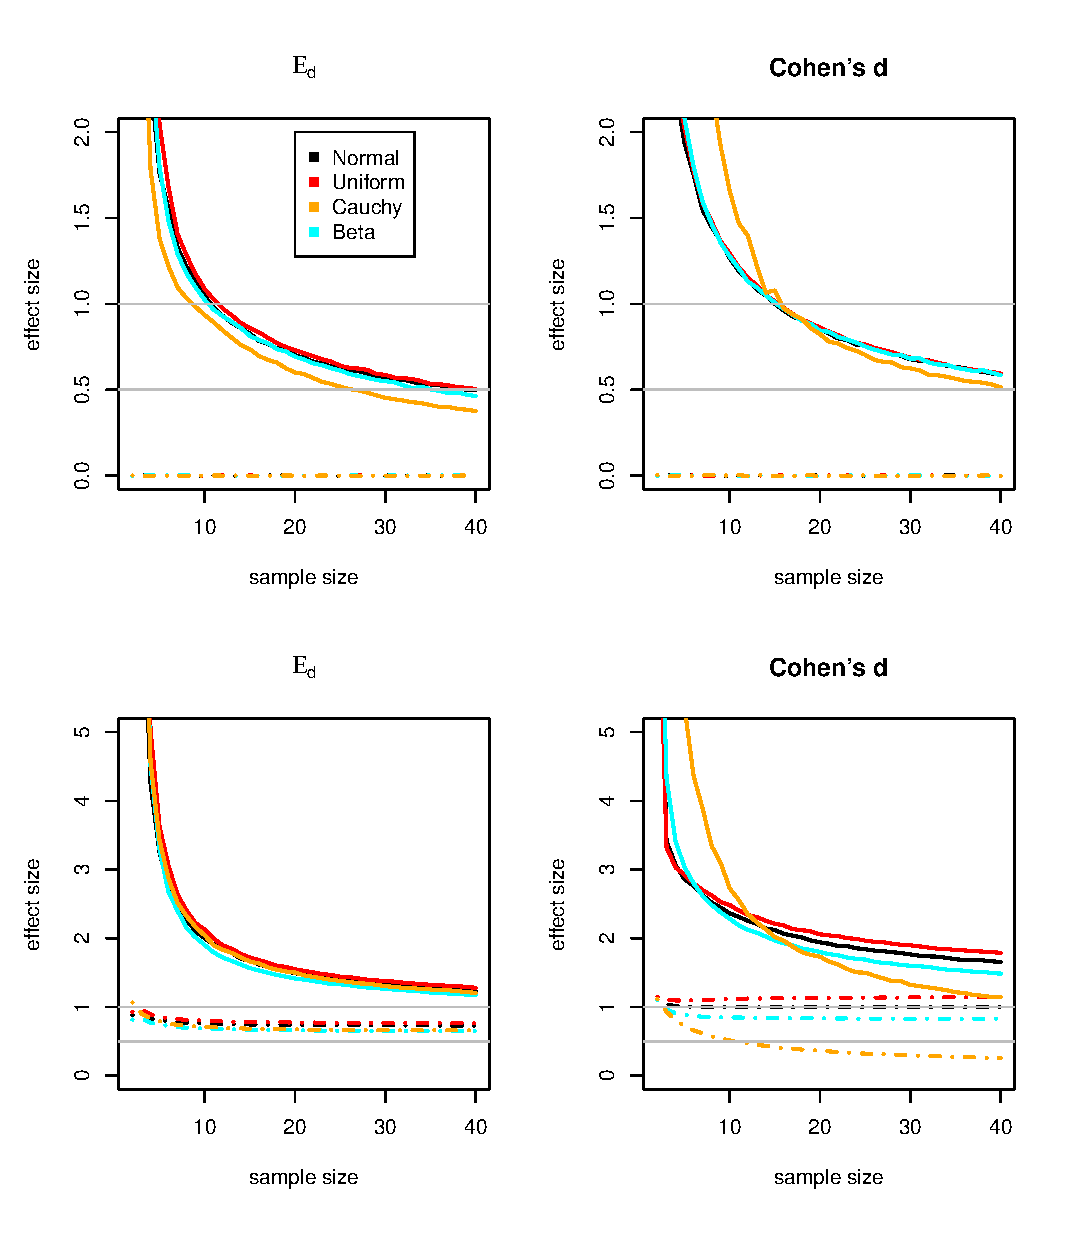
\includegraphics[scale=0.50]{submission/F1-null-model.eps}}
\caption{Characteristics of $\mathcal{E}_{d}$ and when detecting differential features in two groups in random Normal, random uniform, random Cauchy and a heavily skewed random $\beta$ distribution as a function of the per group sample size. The top panels show the behaviour of the $\mathcal{E}_{d}$ and Cohen's~d effect sizes when the two groups are drawn from the same distribution. The simulation included one-hundred thousand random distributions for each. The bottom two panels show the behaviour when there is a difference between groups. Single examples of the distributions are shown in the Supplement. The dashed lines show the median effect size, the solid lines show the 99\textsuperscript{th} percentile of the statistics.  }
\label{fig:01}
\end{figure}

The bottom two panels in Figure \ref{fig:01} show the behaviour when there is a small difference between groups; for reference; Supplementary Figure 5 shows single examples of the distributions used  for comparison.  Again, we can see that the distribution of the median and 99\textsuperscript{th} percentile difference at low sample sizes and are remarkably similar when using the  non-parametric $\mathcal{E}_{d}$ effect size metric, but diverge substantially when using the parametric Cohen's~d. Thus, we conclude that if the data were drawn from a Normal distribution that Cohen's~d would be preferred. However, given that distributions from actual sequencing datasets are unknown, and can be nearly Cauchy, multimodal or skewed \citep{fernandes:2013},  the non-parametric $\mathcal{E}_{d}$ effect size statistic gives a more stable and robust estimate of the standardized difference between distributions than does Cohen's~d.

\begin{figure}[tpb]
\centerline{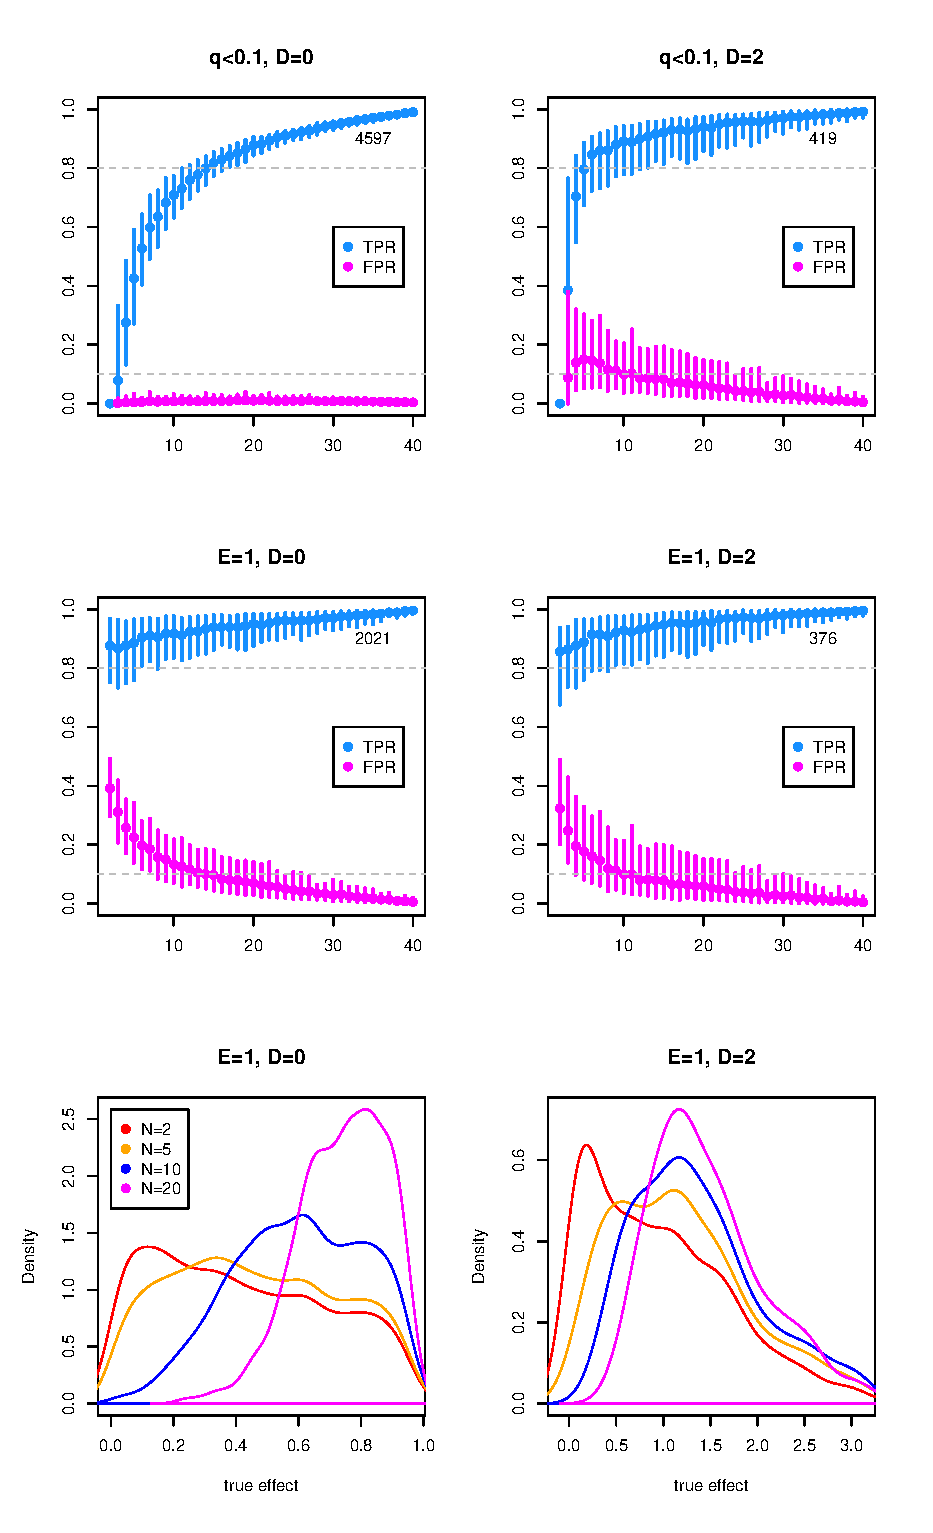
\includegraphics[scale=0.5]{submission/F2-yeast_TPFP.eps}}
\caption{Comparing $\mathcal{E}_{d}$ and adjusted  p-values when detecting differential features between two groups. The top four panels show the   median and 95\% confidence interval of the true positive rate (TPR) and false positive rate (FPR) at different cutoff values.  The top two panels show the values for the q-value, the Benjamini-Hochberg corrected p-value, as a function of sample size. The middle two panels show the values for $\mathcal{E}_{d}$. Data were summarized using either a  0 or 2-fold difference cutoff (D). The number of features of the 6236 non-0 features that are identified as significantly different in the full dataset are shown in the top right corner of each plot. The bottom two panels show the effect size distribution of features identified as false positives by $\mathcal{E}_{d}$ at four different sample sizes. The dashed grey lines show the cutoff for a 10\% FDR and an 80\% power to detect.}
\label{fig:02}
\end{figure}


With this null behaviour information, we can examine an example dataset of a highly replicated RNA-seq dataset geneated by \citep{Schurch:2016aa}. In this dataset, the edgeR tool identified over 4600 out of 6349 genes as `significant'  (Benjamini-Hochberg adjusted p-value $< 0.05$) when all samples were included using either the glm or exact test modes (Supplementary Table 1).  Other widely used tools gave similar results \citep{Schurch:2016aa}. The null hypthesis testing framework in ALDEx2 also returned at least 4300 genes in the same dataset. Thus, identifying such a large proportion of genes as differentially abundant indicates that statistical significance is not informative for this type of experiment. Schurch et al. (and others) recommend adding a secondary threshold such as a fold-change cutoff to identify genes of interest for follow-up analyses \citep{Cui:2003aa,Schurch:2016aa}. When sample sizes are sufficiently large, we would expect that the fold-change cutoff itself would be the primary determinant of difference; however, this approach would not include either the biological variance or the uncertainty of measurement in the analysis.  

\begin{figure}[tpb]
\centerline{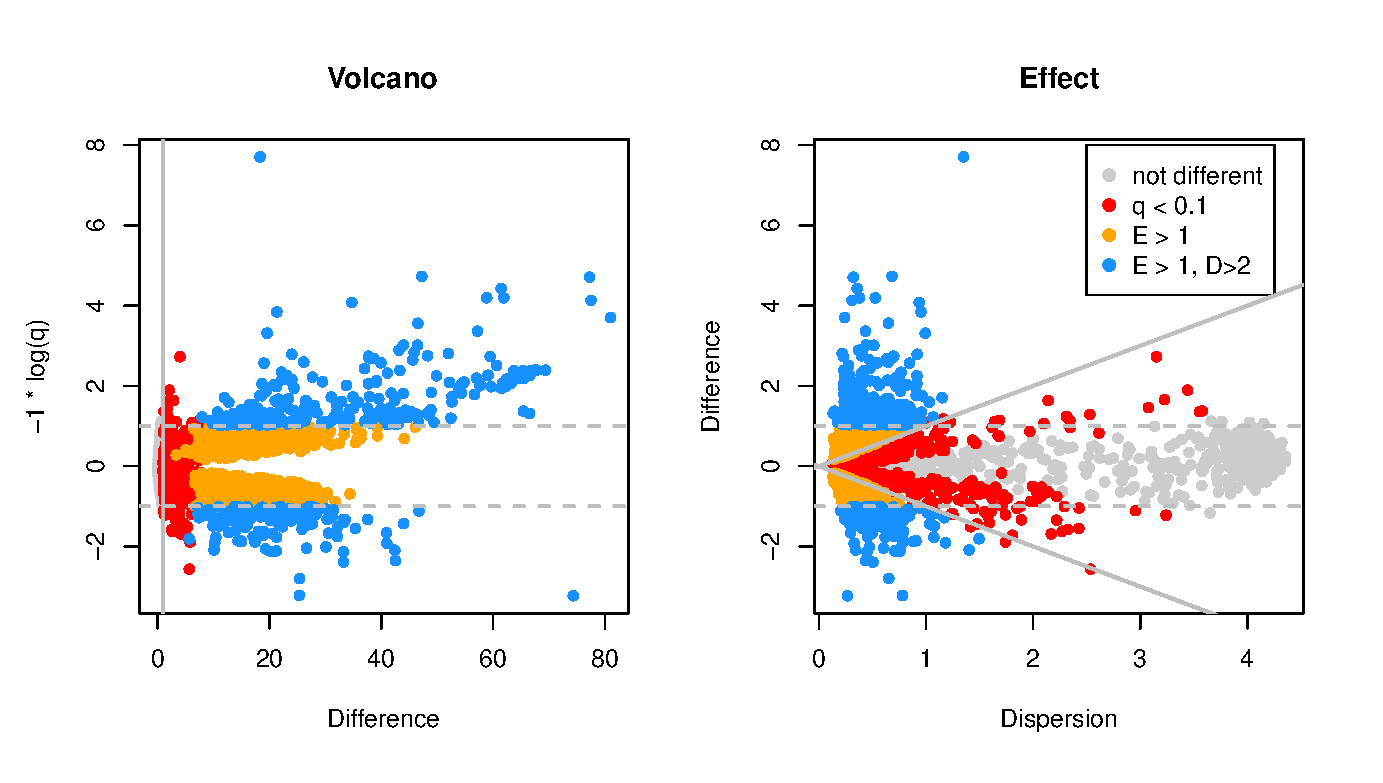
\includegraphics[scale=0.4]{submission/F3-yeast_volcano.eps}}
\caption{Volcano and Effect plots of features identified by  $\mathcal{E}_{d}$,  adjusted p-values  and absolute differences when detecting differential features between two groups. These plots compare the features identified by $\mathcal{E}_{d}$ and by q-scores (FDR) and a 2-fold fold-change thresholds in the full dataset.  In these plots all features that have a q score less than 0.1 also have an effect size greater than 1. Thus, the features in magenta are only identified as significantly different by q scores, those in orange are significantly different by both their q score and their effect size, and features in blue are significant by their q score, their effect size and their absolute difference.  The dashed grey lines in the two plots demarcate the 2-fold difference location; note that the difference is in a log2 scale. The Volcano plot is rotated from its usual orientation and the vertical solid line in the Volcano plot indicates a q score of 0.1. The diagonal solid lines in the Effect plot indicate the boundary where the difference equals the dispersion; ie, where the effect size is 1.
}
\label{fig:03}
\end{figure}

The relationship between sample size and the number of features identified as significantly different using a null hypothesis testing framework in this dataset is shown in the top  panels of Figure \ref{fig:02}.  Here we are testing for the ability to detect all features that would have been observed as differentially expressed in the full dataset when using a random subset of the data. The top two panels were generated using the expected value of the Benjamini-Hochberg corrected Welch's t-test by ALDEx2, but similar plots can be observed using the edgeR tool  or others \citep{Schurch:2016aa}. As expected we observe that the power of a t-test is strongly affected by sample size when the minimum absolute difference between groups is 0. However, when the minimum feature difference is a 2-fold change (D=2), the number of features identified is reduced approximately 10 fold, and a relatively small number of samples is required for acceptable power. The tradeoff here is that applying both the q-score and difference cutoffs results in an increase in the FDR at small numbers of samples. Note that all tools have difficulty estimating the actual FDR in many datasets \citep{Thorsen:2016aa,hawinkel2017}. 

The middle two panels of Figure \ref{fig:02} show the behaviour of the $\mathcal{E}_{d}$ statistic in the same random datasets. Note that even when only two samples are used, the $\mathcal{E}_{d}$ statistic identifies over 80\% of the features as different as are identified by the same statistic in the full dataset. Thus, the simple metric outlined here  can correctly identify the `true positive' set even when the number of samples is very small. The tradeoff when using this statistic is that at very low sample sizes the False Discovery Rate (fdr) is extreme; in this dataset and with and with a cutoff of $\mathcal{E}_{d} > 1$, the fdr is 40\% with two samples, but falls to less than 10\% only when there are 15 or more samples. Interestingly, applying a fold-change cutoff to the $\mathcal{E}_{d}$ metric reduces the false discovery rate dramatically and also reduces the number of features identified as significantly different. 

The bottom two panels of Figure \ref{fig:02} show the effect size in the full dataset of false positive features identified as different in subsets of the dataset. We can see that at a sample size of 2 the false positive features have true effect-sizes that are nearly randomly distributed, but that at a sample size of 10 or more, the vast majority of false positive features have true effect sizes that are at least 50\% of the desired effect size. When applying the difference cutoff, we observe that the majority of false positive features identified at small sample sizes have an effect size greater than the cutoff when the sample size is 5 or more. Thus, this implies that false positive features in this case pass the effect size cutoff but fail on the absolute difference cutoff. Supplementary Figure 6 shows a similar analysis for a 16S rRNA gene sequencing dataset \citep{bian:2017} with similar results, even thought he abundance/variance relationship between the features is very different than in the transcriptome experiment (Supplementary Figure 7). Supplementary Figure 8 shows that the effect thresholds from the simulated data in Figure 1 are appropriate, and perhaps even conservative, for real HTS data, and provide further evidence that the features identified as different in Figure 2 are likely to be reproducible.

Taking the data from Figures \ref{fig:01} and \ref{fig:02}, and the Supplement together, we can provide guidance as to appropriate cutoff values when using the $\mathcal{E}_{d} $ statistic in HTS datasets. First,  point estimates of $\mathcal{E}_{d} $ in real datasets and in simulated distributions are highly congruent. Thus, we can estimate that for every 100 features in a HTS dataset, we can use the curves in Figures \ref{fig:01} and  Supplementary Figure 8 to determine the number of false positive features expected if there is truly no difference between groups. The CoDaSeq R package contains a function that can be used to empirically determine thresholds for any desired percentile cutoff. As an example, the plots in Figure \ref{fig:01} that as a rule of thumb for the experimentalist to be 99\% confident in a true positive, effect sizes should be greater than 2 when the sample size is  4, greater than 1 when the sample size is 10, and greater than 0.5 for sample sizes larger than 40. This rule of thumb holds true regardless of the true underlying distribution and is appropriate whenever point estimates are computed. When computing the expected $\mathcal{E}_{d} $ as does the aldex.effect function, these thresholds are much lower at small sample sizes, and effect sizes can be about 30\% smaller. 

Figure \ref{fig:03} shows how the different threshold cutoffs relate to each other when plotted as a difference vs. q-score in a Volcano plot \citep{Cui:2003aa} and in a dispersion vs difference Effect plot \citep{gloor:effect}. These plots demonstrate the advantage of using a standardized effect metric over a q-score either with or without an absolute difference cutoff. In the Volcano plot, the q-score only features coloured in magenta, are exclusively features that have q scores near the upper bound of statistical significance. These include features with both large and small absolute differences, and the reason that a feature may have a large difference but a marginally significant q-score is not revealed on the Volcano plot. However, examination of the Effect plot shows that features that have a marginal q-score and large difference are features with very large dispersion; that is the difference between features, $\tilde{D}$, is much smaller than the within-group dispersion, MMAD, calculated as in Equation \ref{eq:ff}. Such features would not be expected to reproduce well in a new dataset because of their intrinsically high variance. In fact, these features are exactly those that are excluded by the $\mathcal{E}_{d} $ statistic.  Furthermore, adding the constraint that features have at least a 2-fold difference does not exclude these high-dispersion features from consideration. 

Examination of the orange features in the Volcano and Effect plots, we can see that both q-scores and $\mathcal{E}_{d} $ can exhibit arbitrarily small absolute differences if the dispersion is very small. In the case of the $\mathcal{E}_{d} $ statistic, adding in the requirement for at least a 2-fold change reduces the number of features to only those that are both different and reproducible.  
